%参考网站:http://tex.stackexchange.com/questions/42812/3d-bodies-in-tikz
\documentclass[tikz,border=2pt]{standalone}

\usetikzlibrary{3d,calc}

\begin{document}

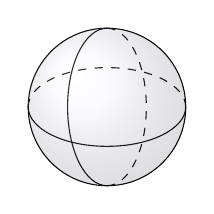
\begin{tikzpicture}
    \draw (-1,0) arc (180:360:1cm and 0.5cm);
    \draw[dashed] (-1,0) arc (180:0:1cm and 0.5cm);
    \draw (0,1) arc (90:270:0.5cm and 1cm);
    \draw[dashed] (0,1) arc (90:-90:0.5cm and 1cm);
    \draw (0,0) circle (1cm);
    \shade[ball color=blue!10!white,opacity=0.20] (0,0) circle (1cm);
\end{tikzpicture}

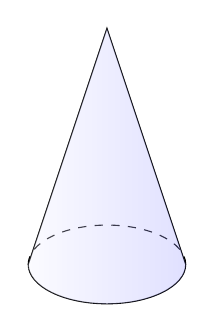
\begin{tikzpicture}
    \draw (-1,0) arc (180:360:1cm and 0.5cm) -- (0,3) -- cycle;
    \draw[dashed] (-1,0) arc (180:0:1cm and 0.5cm);
    \shade[left color=blue!5!white,right color=blue!40!white,opacity=0.3] (-1,0) arc (180:360:1cm and 0.5cm) -- (0,3) -- cycle;
\end{tikzpicture}

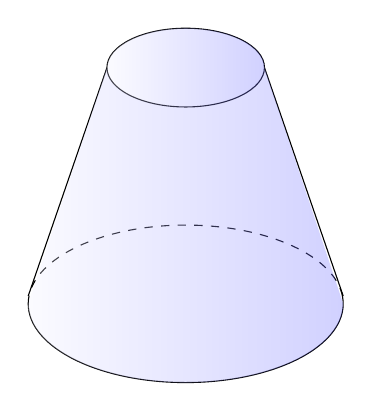
\begin{tikzpicture}
    \draw (-1,0) arc (180:360:1cm and 0.5cm);
    \draw (-1,0) arc (180:0:1cm and 0.5cm);
    \draw (-2,-3) arc (180:370:2cm and 1cm);
    \draw[dashed] (-2,-3) arc (180:10:2cm and 1cm);
    \draw(-2,-2.9)  -- (-1,0);
    \draw(2,-2.9)   -- (1,0);
    \shade[left color=blue!5!white,right color=blue!60!white,opacity=0.3] (-1,0) arc (180:360:1cm and 0.5cm) -- (2,-3) arc (360:180:2cm and 1cm) -- cycle;
    \shade[left color=blue!5!white,right color=blue!60!white,opacity=0.3] (0,0) circle (1cm and 0.5cm);
\end{tikzpicture}

\end{document}
